\chapter{ADU}

\section{Aufgabe 23}

\paragraph*{}
In dieser Aufgabe soll der Wert einer externen Spannungsquelle gemessen werden und dann anschlißend über die serille Schnittstelle an den PC übermittel werden. Zu erst initialsieren wir den Spannungswandler, und geben als obere bzw. untere Referenzspannung 3V bzw 0V an. Anschlißend konfigurieren wir den Timer so das wir Abstand von einer Sekunde benachrichtigt werden. Die ISR signalsiert uns, wann wir eine Wandlung anstoßen sollen, dies minimiert den Code in der ISR. Allerdings kann dies dazuführen das wir eine neue Wandlung starten bevor die alte abgeschlossen ist (dieser Fall kann jedoch abgefangen werden, durch lesen des {\em ADC12BUSY}-Bits,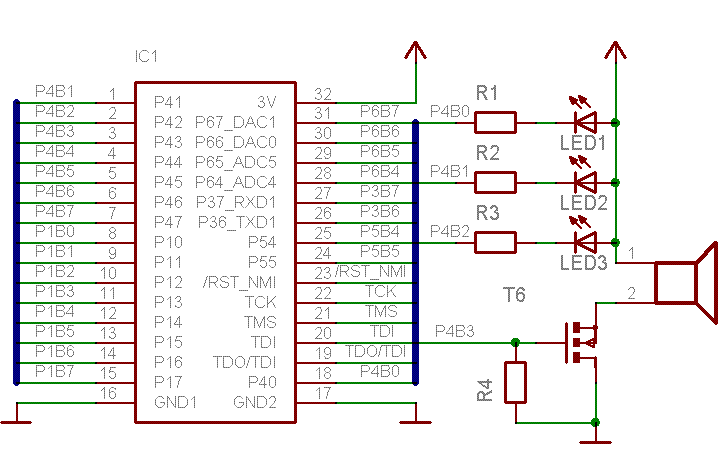
\includegraphics[width=\textwidth]{img/mikrocontrollerUNDled.png} welches angibt ob die Wandlung abgeschlossen wurde).

\lstinputlisting[caption=intterrupts.c für Aufgabe 23]{src/interrupts_aufgabe23.c}

\paragraph*{}
Als Ergebnis der Wandlung erhalten wir einen 12-bit langen Integerwert. Dabei steht der Wert 4096 für unsere obere und 0 für die untere Refrenzspannung. Dazwischen sind die Werte lineare verteilt. Durch eine einfache Rechnung erhalten wir den Wert in Volt und geben ihn anschließend auf der Konsole aus.

\lstinputlisting[caption=aufgabe23.c]{src/aufgabe23.c}

\section{Aufgabe 24}

\paragraph*{}
Im Hauptprogramm initialsieren wir den ADU und den TimerB um regelmäßig Wandlung durch zu führen. Dabei gehen wir weitgehend analog zu vorherigen Aufgabe vor. In der Endlosschleife warten wir auf einen Aufruf der Timer-ISR und starten eine Wandlung sobald diese unse signalsiert. 
\lstinputlisting[caption=aufgabe24.c]{src/aufgabe24.c}

\paragraph*{}
Wir nutzen die ISR des AD-Wandlers. Diese wird aufgerufen sobald die Wandlung abgeschlossen ist. Da der Prozessor über mehrer AD-Wandler verfügt können wir alle Werte aufeinmal wandeln und diese anschlißend auf die serielle Konsole schreiben.  

\lstinputlisting[caption=intterrupts.c für Aufgabe 23]{src/interrupts_aufgabe23.c}

\paragraph*{}
Als Ergbeniss erhalten wir drei Kurven, die sich in Abhänigkeit von der Bewegung des Kontrollers ändern. Die z-Achse misst durchgehend höhre Werte, da sie die Erdbeschleunigung mit misst.

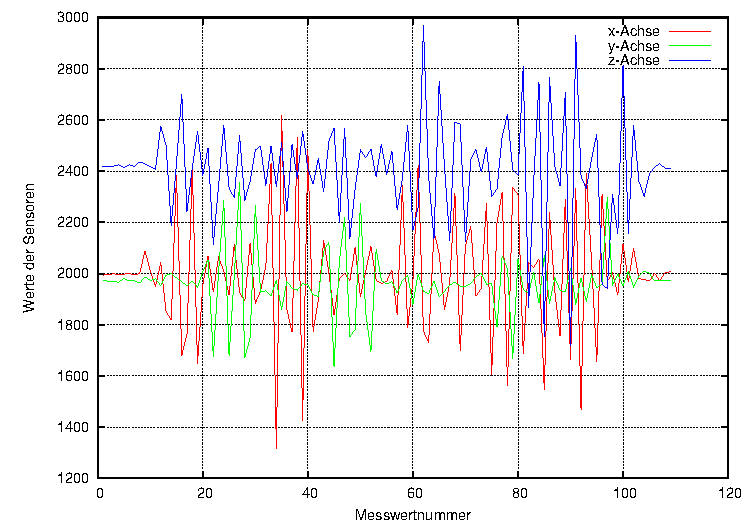
\includegraphics[width=\textwidth]{graphs/accel.pdf}

